\chapter{Resultados y An\'{a}lisis}
A continuaci\'{o}n se presentan como datos originales de este documento de tesis, los resultados de algunas propiedades globales, como lo es el coeficiente de difusi\'{o}n y el perfil de estr\'{e}s de la membrana. Tambi\'{e}n se presentan algunas propiedades medidas a nivel local, como es el \'{a}rea por l\'{i}pido local y el espesor de la membrana local. El constante de difusi\'{o}n fue obtenido con las herramientas de gromacs, el perfil de estr\'{e}s fue hallado con la herramienta mdstress, mientras que el \'{a}rea por l\'{i}pido y el espesor con g\_lomepro. Para los resultados de g\_lomepro se obtienen tambi\'{e}n distribuciones y promedios que se pueden comparar con las propiedades globales presentadas en el cap\'{i}tulo anterior.\\

\section{Propiedades Locales de los Compuestos de la Membrana}
% \subsection*{Par\'{a}metros del grupo \ce{O1-C22-C23-C24}}
\subsection*{Par\'{a}metros de la cadena diaponeurosporenoica desde \ce{C23} hasta \ce{C47}}


Para verificar si el complejo de enlaces dobles conjugados permanece en conformaci\'{o}n \textit{trans}, se realizaron histogramas del \'{a}ngulo dihedral sobre las simulaciones realizadas. En la figura \ref{fig:dihdist} aparecen los histogramas para los  \'{a}ngulos dih\'{e}dricos a partir del \ce{C23}, el primer enlace aparece en la estructura molecular como \ce{C23=C24-C25=C26}, el siguiente como \ce{C24-C25=C26-C27} y as\'{i} sucesivamente hasta llegar a \ce{C38=C39-C40=C41}. Adicicionalmente, en la figura \ref{fig:dihavg} parecen los valores medios y los errores est\'{a}ndares de cada una de estas distribuciones. En este complejo de enlaces dobles conjugados, se observa que en promedio la cadena se mantiene en una estructura \textit{trans}, puesto que los picos de las distribuciones est\'{a}n cerca a $\pm 180^{\circ}$, sin embargo hay ciertas fluctuaciones debidas a la agitaci\'{o}n entre las mol\'{e}culas, las cuales entran dentro del error est\'{a}ndar. Tambi\'{e}n se observa que el \'{a}ngulo dihedral \ce{C39-C40=C41-C43} permanece en posici\'{o}n \textit{trans}.\\
\begin{figure}[t]
\begin{center}
    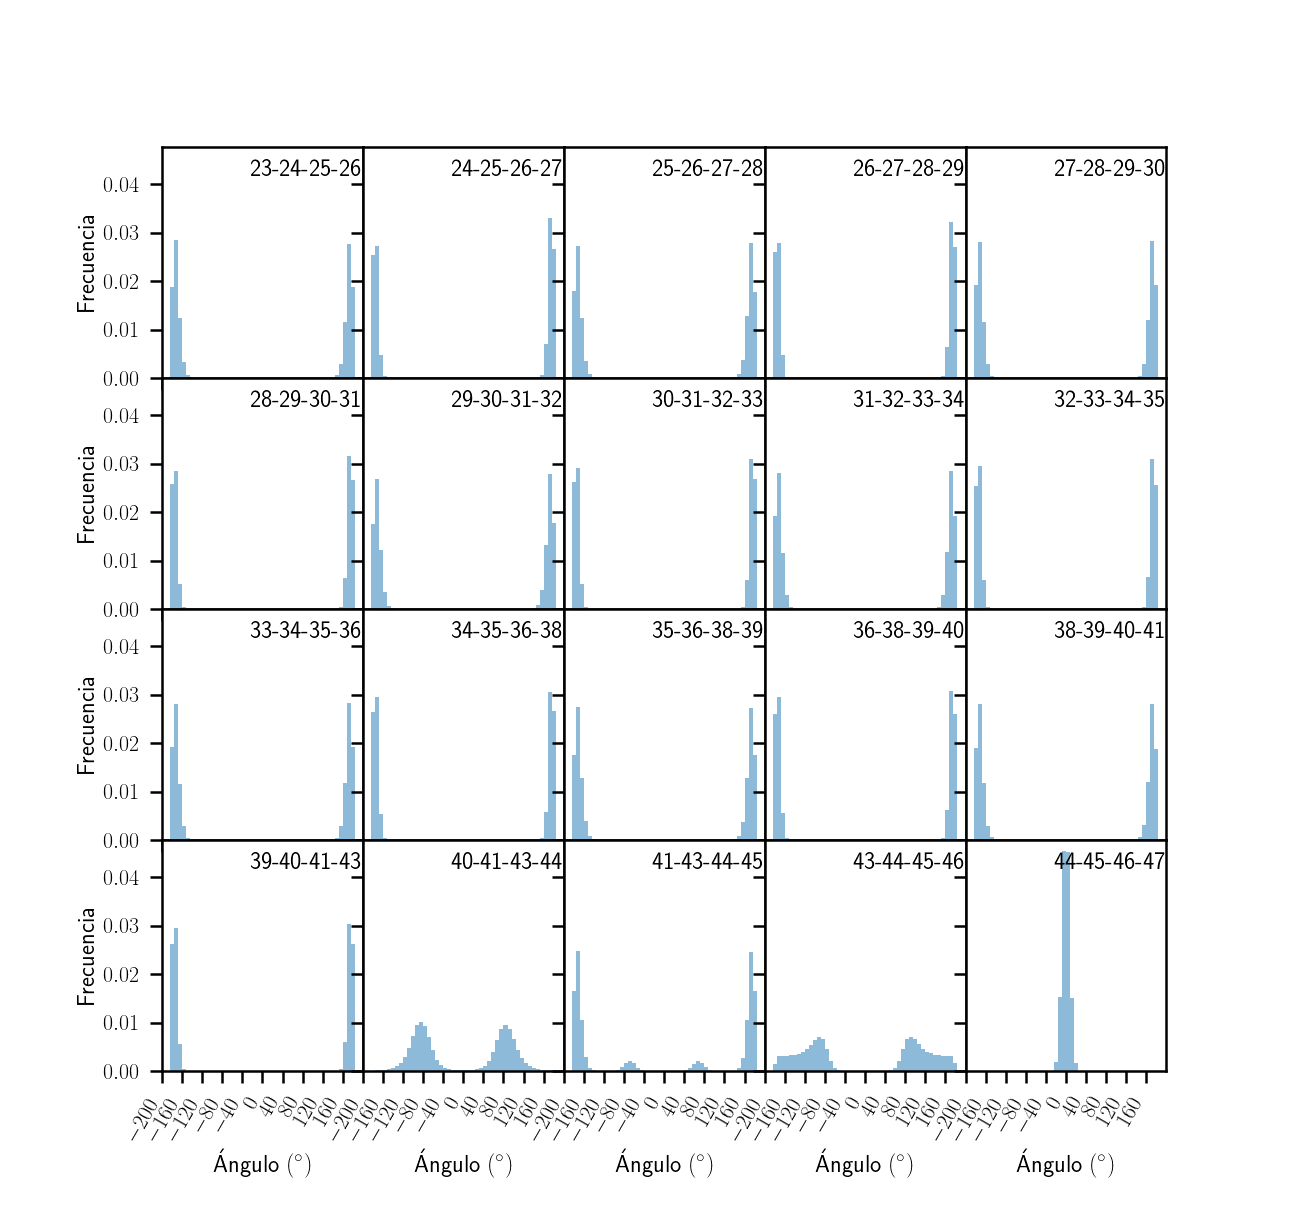
\includegraphics[scale=0.32,trim={0 3cm 0 4cm},clip]{Plots/dihedral_15STX-DMPG.png}
  \caption{Distribuci\'{o}n de los \'{a}ngulos dih\'{e}dricos de la cadena diaponeurosporenoica para el sistema 15\%STX en DMPG. Los dem\'{a}s sistemas presentan pr\'{a}cticamente las mismas distribuciones.}
  \label{fig:dihdist}
\end{center}
\end{figure}
\begin{figure}
\begin{center}
    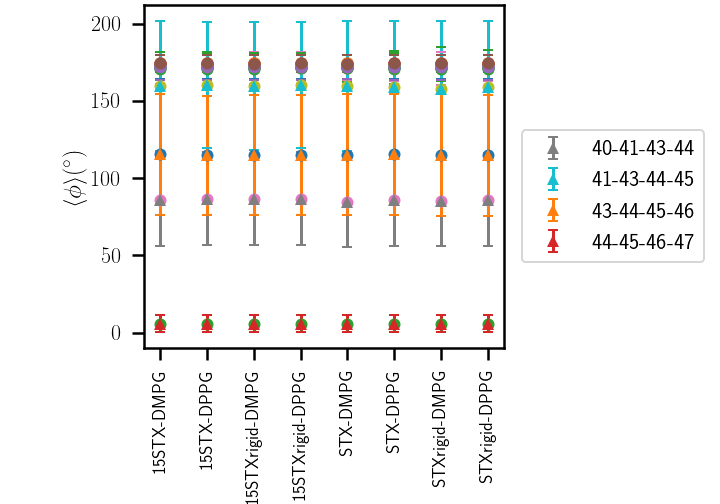
\includegraphics[scale=0.4]{Plots/dihedrals.png}
  \caption{Promedios temporales y espaciales (en valor absoluto) de los \'{a}ngulos dih\'{e}dricos de la cadena diaponeurosporenoica para todos los sistemas simulados. Los puntos caf\'{e}s y morados de la parte de arriba son los promedios para los dihedros entre \ce{C23} y \ce{C43}. Los dem\'{a}s colores son para los dihedros restantes.}
  \label{fig:dihavg}
\end{center}
\end{figure}

Por el contrario, se encuentran distribuciones distintas para los \'{a}ngulos dihedrales  de los \'{a}tomos \ce{C40=C41-C43-C44}, \ce{C41-C43-C44-C45} , \ce{C43-C44-C45=C46} y \ce{C44-C45=C46-C47}. En todos los 4 casos, las distribuciones son m\'{a}s anchas. Esto nos indica que esta regi\'{o}n de la estafiloxantina es m\'{a}s m\'{o}vil y puede acomodarse m\'{a}s f\'{a}cil dentro de la membrana comparada con su regi\'{o}n de enlaces dobles conjugados. En los casos \ce{C40=C41-C43-C44} y \ce{C43-C44-C45=C46} aparecen regiones prohibidas para las conformaciones \textit{cis} ($\phi=0^{\circ}$) o \textit{trans} ($\pm\phi=180^{\circ}$) y, esto puede deberse a una ramificaci\'{o}n en la posici\'{o}n \ce{C41} lo cual puede generar impedimentos est\'{e}ricos que dificulten ubicar esta regi\'{o}n en posici\'{o}n \textit{cis} o \textit{trans}.  El caso \ce{C41-C43-C44-C45} es el que presenta en promedio una orientaci\'{o}n m\'{a}s trans comparada con los otros tres dihedros. A pesar de esto, tambi\'{e}n posee dos picos m\'{a}s peque\~{n}os en una orientaci\'{o}n intermedia, indicando que hay menos certeza en ubicar al dihedro en una sola conformaci\'{o}n. Finalmente, para el dihedro \ce{C44-C45=C46-C47} se observa una contundente conformaci\'{o}n cis, que dentro del error alcanza a caer en las d\'{e}cimas de grado. Esto se debe a que en la punta de la cadena la estafiloxantina tiene dos ramificaciones, las cuales restringen de forma simul\'{a}nea su movimiento. En general, los resultados de libertad rotacional en los \'{u}ltimos carbones de la cadena diaponeuroesporenoica indican que el segmento final puede adoptar varias conformaciones, lo cual debe influir fuertemente en la organizaci\'{o}n de la mol\'{e}cula dentro de la membrana. Es interesante notar que otros carotenoides bacterianos no presentan esta libertad rotacional en los carbones terminales debido a que los enlaces dobles conjugados es mantienen hasta el final de la cadena. Ser\'{i}a de interes entender por qu\'{e} evolutivamente se rompe el patr\'{o}n de enlaces conjugados para esta mol\'{e}cula y si cumple alguna funci\'{o}n estructural.\\

\subsection{\'{A}rea Local por L\'{i}pido}
Mediante la herramienta de g\_lomepro se obtuvo el \'{a}rea local por l\'{i}pido para todos los sistemas. En la figura \ref{fig:aplsnap} se muestra como se distribuye el \'{a}rea por l\'{i}pido sobre las monocapas inferiores y superiores de la membrana para los sistemas a) 15\% STX-DMPG, b) la membrana pura de DMPG, c) y d) monocapas superior e inferior de 1STX:128DMPG. En el anexo \ref{AnexoA} adem\'{a}s aparecen los perfiles de las \'{a}reas locales para todos los sistemas estudiados. En las figuras mostradas la membrana se ha dividido en una grilla de $50\times 50$ tanto en la monocapa superior como en la inferior. Adicionalmente las escalas aparecen en la parte inferior de cada figura, entre m\'{a}s rojo es mayor el APL, entre m\'{a}s azul es menor el APL.\\ 

\begin{figure}
\begin{center}
    \includegraphics[scale=0.04]{Plots/snap_15STX-DMPG_1_up.png}
    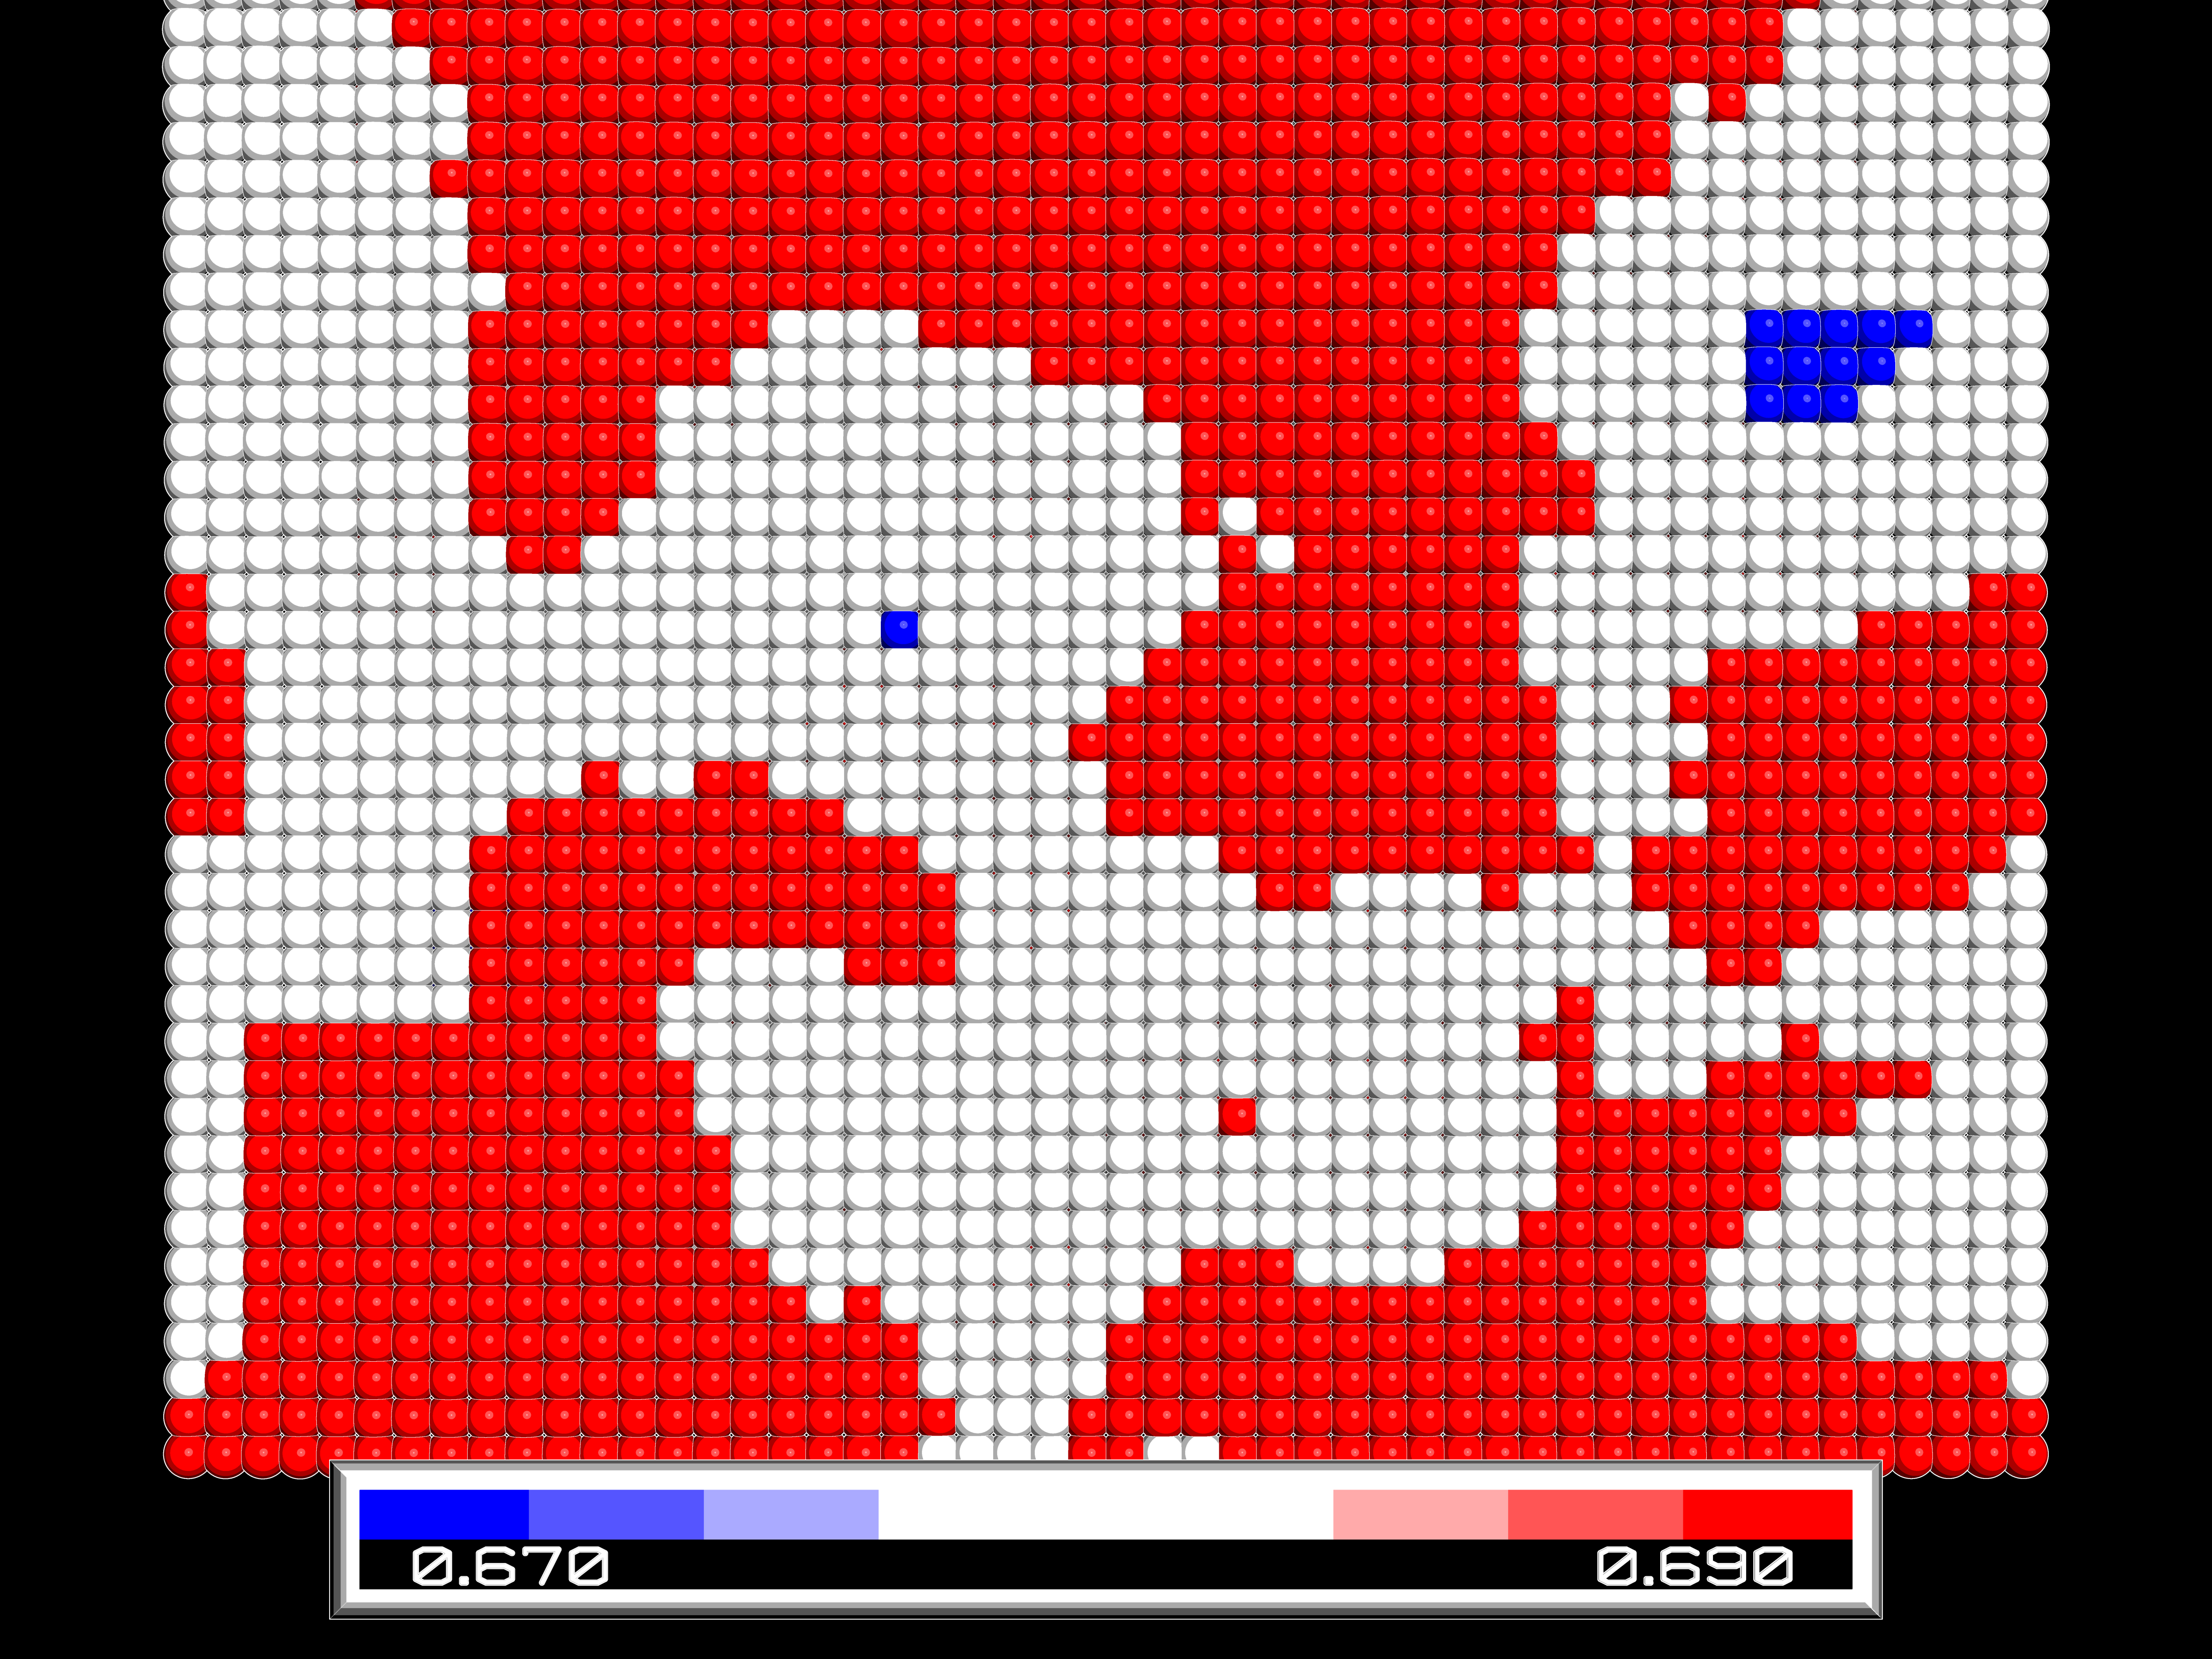
\includegraphics[scale=0.04]{Plots/snap_MEM-DMPG_1_up.png}
    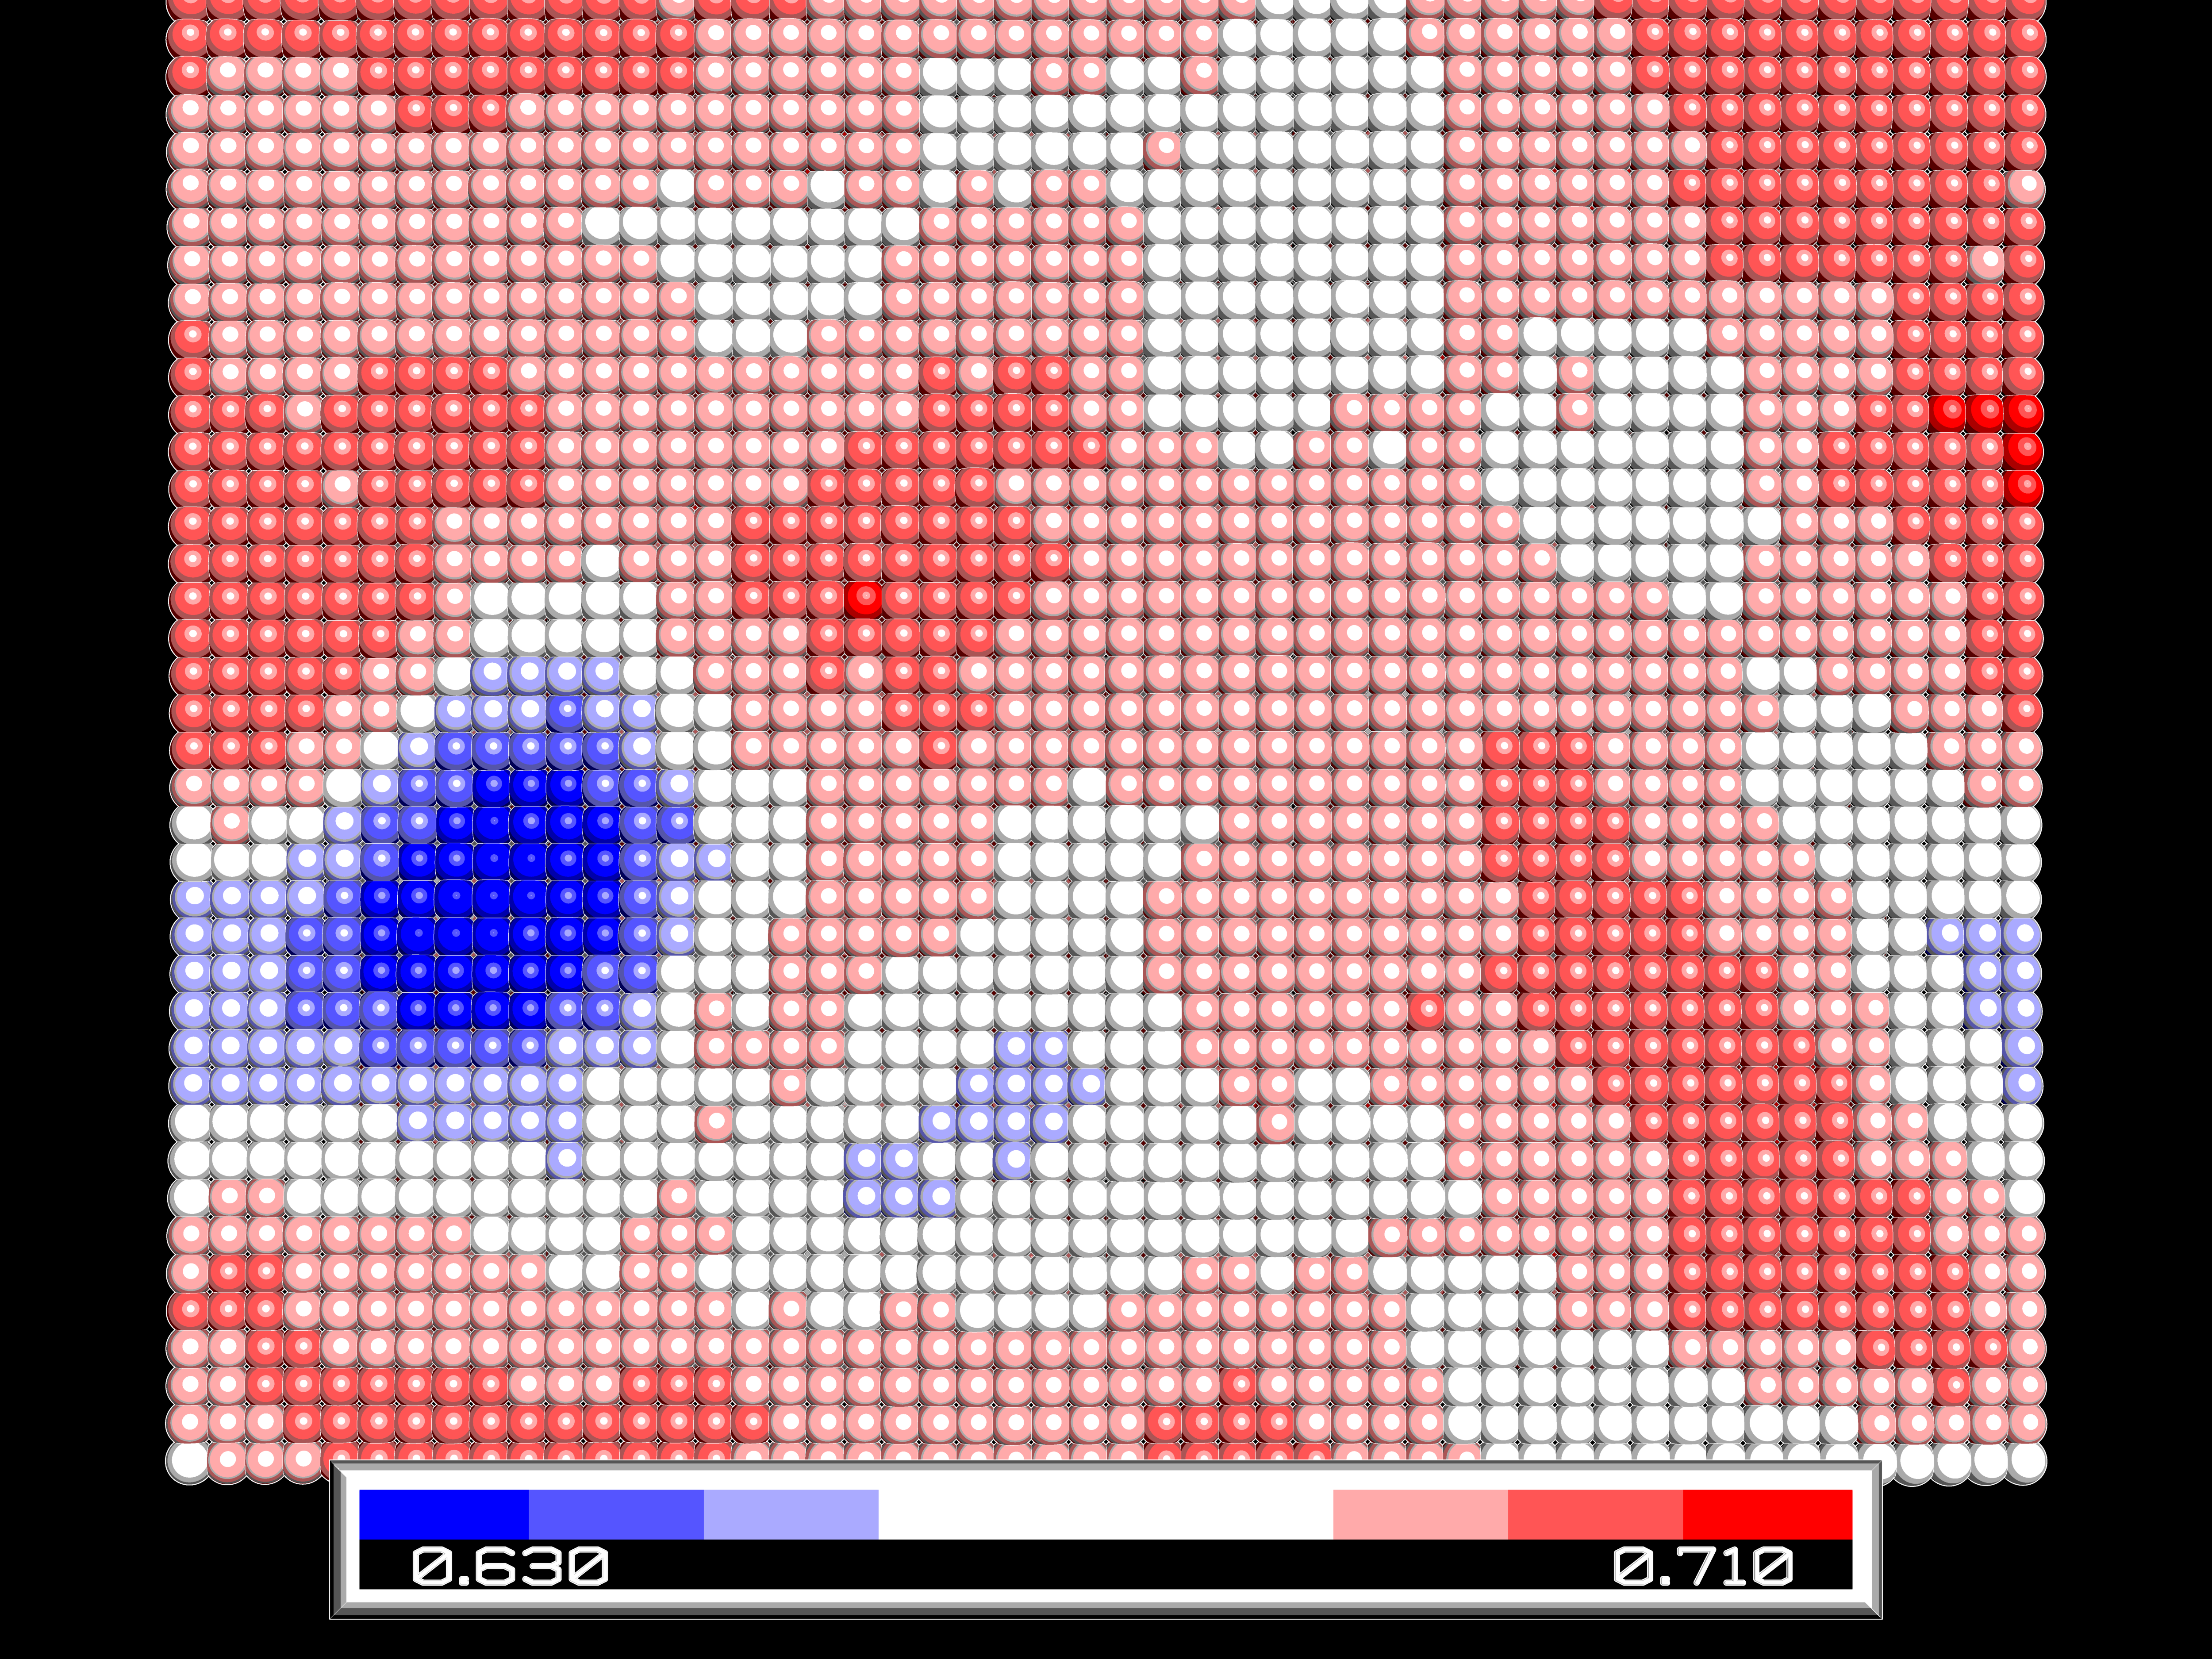
\includegraphics[scale=0.04]{Plots/snap_STX-DMPG_1_up.png}
        \includegraphics[scale=0.04]{Plots/snap_STX-DMPG_1_do.png}
    % \put(-130,80){a)}
    % \put(-130,50){b)}
    % \put(-130,20){c)}
    % \put(-130,20){d)}
  \caption{Representaci\'{o}n de el \'{a}rea por l\'{i}pido local. \textit{Arriba izq.}: El sistema 15\% STX-DMPG, \textit{Arriba der.}: Membrana pura de DMPG, \textit{Abajo izq.}: 1STX:128DMPG en la monocapa superior (donde est\'{a} el az\'{u}car de STX y\textit{Abajo der.}: 1STX:128DMPG en la monocapa inferior. Figura obtenida con g\_lomepro y PyMol.}
  \label{fig:aplsnap}
\end{center}
\end{figure}
\begin{table}
\centering
\begin{tabular}{|c|c|c|}
\toprule
{} &  $\mathbf{\langle A\rangle(n\mathrm{m}^{2})}$ &  $\mathbf{\Delta A(n\mathrm{m}^{2})}$ \\
\midrule
\textbf{15STX-DMPG     } &            0.64 &        0.03 \\
\textbf{15STX-DPPG     } &            0.62 &        0.03 \\
\textbf{15STXrigid-DMPG} &            0.64 &        0.03 \\
\textbf{15STXrigid-DPPG} &            0.62 &        0.03 \\
\textbf{MEM-DMPG       } &            0.66 &        0.00 \\
\textbf{MEM-DPPG       } &            0.64 &        0.00 \\
\textbf{STX-DMPG       } &            0.66 &        0.01 \\
\textbf{STX-DPPG       } &            0.64 &        0.01 \\
\textbf{STXrigid-DMPG  } &            0.66 &        0.01 \\
\textbf{STXrigid-DPPG  } &            0.64 &        0.01 \\
\bottomrule
\end{tabular}
\caption{Valores de \'{a}reas locales por l\'{i}pido obtenidas para cada uno de los sistemas.}
    \label{tab:aplglomepro}
\end{table}
En la figura \ref{fig:aplsnap} se observa que en los sistemas con 15\%mol STX aparecen regiones uniformes con mayores y menores \'{a}reas por l\'{i}pido, mientras que para el sistema de una sola estafiloxantina, en la monocapa superior aparece una regi\'{o}n con menor \'{a}rea por l\'{i}pido y el resto de mayor \'{a}rea por l\'{i}pidos. Esto indicar\'{i}a que la estafiloxantina ocupa un \'{a}rea por l\'{i}pido menor a los fosfogliceroles. En la monocapa inferior en cambio, la grilla muestra una \'{a}rea por l\'{i}pido m\'{a}s uniforme en ausencia de cabezas polares de estafiloxantina. El \'{a}rea por l\'{i}pido de menor tama\~{n}o de estafiloxantina, comparado con los fosfogliceroles puede explicarse por la cabeza polar de este l\'{i}pido. Estructuralmente, la glucosa en estafiloxantina toma el lugar del glicerol primario (backbone) en los fosfogliceroles al actuar como la mol\'{e}cula conectora de los dos \'{a}cidos grasos en estafiloxantina. La glucosa es el \'{u}nico grupo polar de estafiloxantina y es peque\~{n}o en tama\~{n}o. En cambio, los fosfogliceroles tienen unido al glicerol primario un grupo fosfato con una carga neta de -1 y un segundo glicerol lo cual resulta en una cabeza polar mas grande. Adicionalmente la carga desnuda del grupo fosfato probablemente induce niveles de hidrataci\'{o}n mayores de las cabezas de los fosfogliceroles y la presencia de contraiones. Estos factores en conjunto explican el mayor tama\~{n}o de las cabezas polares de los fosfogliceroles comparado con estafiloxantina. \\

Con las \'{a}reas locales tambi\'{e}n se hallaron las distribuciones y los valores medios del \'{a}rea por l\'{i}pido. Las distribuciones se muestran en la figura  \ref{fig:aplglomepro} y en la tabla \ref{tab:aplglomepro} aparecen los valores del \'{a}rea por l\'{i}pido obtenidos en promedio para cada uno de los sistemas analizados, el error est\'{a}ndar se obtuvo asumiendo que los datos convergen a una distribuci\'{o}n normal y tomando como aceptables el primer 68\% de los datos alrededor del promedio. \\
\begin{figure}
\begin{center}
    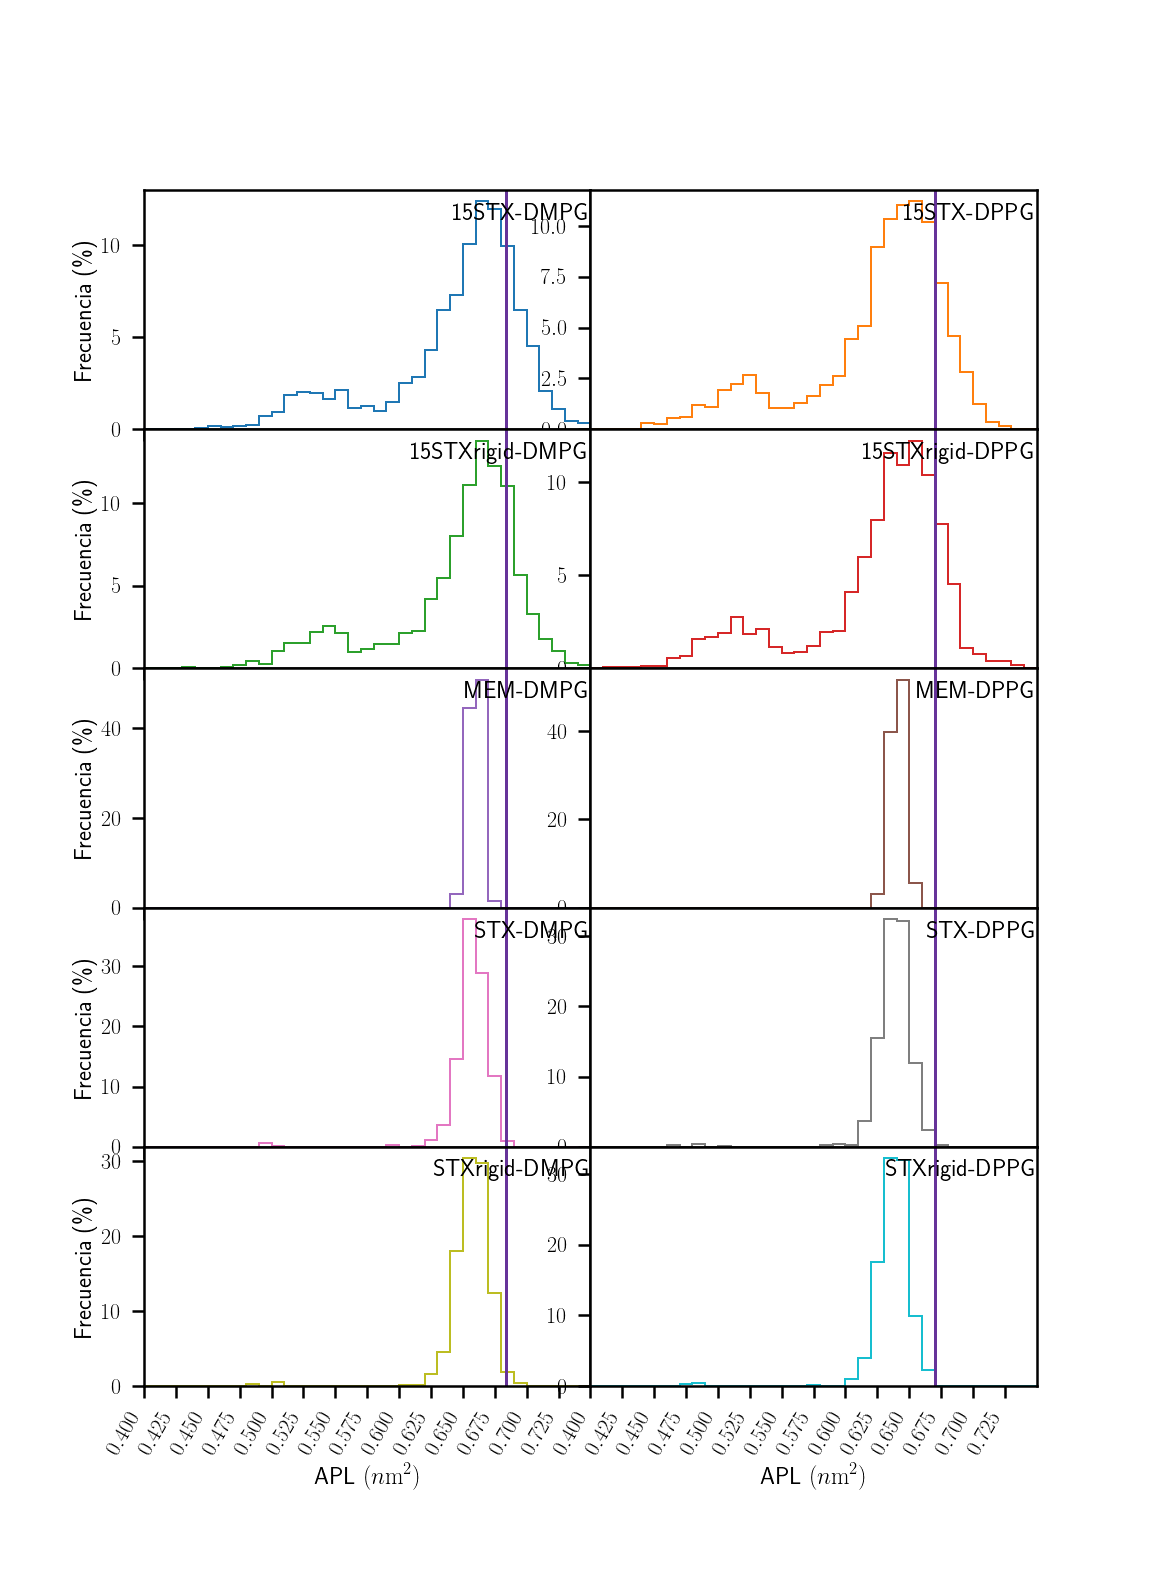
\includegraphics[scale=0.3,trim={0 3cm 0 6cm},clip]{Plots/APL_hist_lipids_g_lomepro.png}
  \caption{Distribuciones del \'{a}rea por l\'{i}pido local halladas con g\_lomepro y para todos los sistemas. Las l\'{i}nas p\'{u}rpura son los valores experimentales encontrados en Pan et. al. \cite{Pan2012}.}
  \label{fig:aplglomepro}
\end{center}
\end{figure}

En las distribuciones aparecen dos poblaciones: Una para las STX y otra para los l\'{i}pidos. Para los sistemas con un 15\% de STX, las estafiloxantinas son las que presentan una menor \'{a}rea por l\'{i}pido, con un pico m\'{a}s abajo en la distribuci\'{o}n, el cual se encuentra alrededor de $0.57n\mathrm{m}^2$ para 15\%STX:DMPG y alrededor de $0.57n\mathrm{m}^2$ para 15\%STX-DPPG. Esto confirma lo observado visualmente en la figura anterior. Con respecto a los picos m\'{a}s grandes  que corresponden a los fosfol\'{i}pidos, estos est\'{a}n dentro del ancho de la distribuci\'{o}n superior y dentro de los valores experimentales, mostrados en la l\'{i}nea morada. En cuanto a los sistemas de membranas puras se observa tanto en la grilla como en las distribuciones que el \'{a}rea por l\'{i}pido presenta una variaci\'{o}n baja,  la cual hace que el valor experimental (l\'{i}nea p\'{u}rpura) no est\'{e} dentro la incertidumbre.\\

En la figura \ref{fig:apl_thickavglomepro} aparecen los valores promedio de las distribuciones del \'{a}rea por l\'{i}pido para g\_lomepro. En las figuras se observa que, acorde con Pan et. al. \cite{Pan2012}, el \'{a}rea por l\'{i}pido para membranas con DMPG es mayor que para membranas con DPPG. Sin embargo, los valores para membranas puras no coinciden con los valores reportados por Pan et. al. \cite{Pan2012}. Cuando se inserta la estafiloxantina se observa que a mayor concentraci\'{o}n de estafiloxantina, menor es el valor promedio del \'{a}rea por l\'{i}pido (sin mirar la incertidumbre), sin embargo, la distribuci\'{o}n  ampl\'{i}a su rango de valores, con lo cual el error incrementa y por lo tanto, los l\'{i}pidos alcanzan los valores para las membranas puras, as\'{i} como tambi\'{e}n el valor experimental.\\
\begin{figure}
\begin{center}
    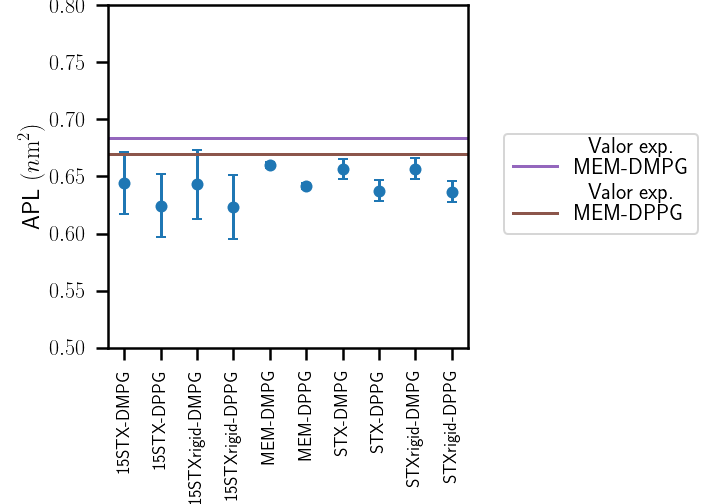
\includegraphics[scale=0.3]{Plots/apl_av_g_lomepro.png}
     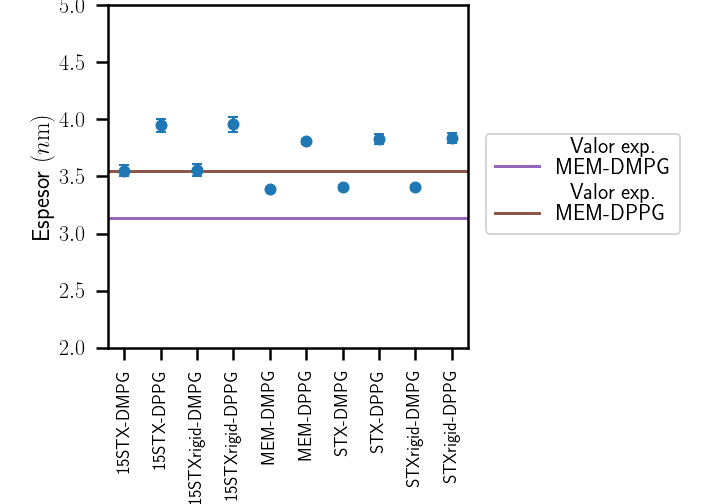
\includegraphics[scale=0.3]{Plots/thickness_average.png}
  \caption{\textit{Izquierda}: Valores promedio del \'{a}rea por l\'{i}pido local, \textit{derecha}: Valores promedio del espesor local  hallados con g\_lomepro para todos los sistemas. Los puntos azules son los valores promedio, mientras que las l\'{i}neas son los valores experimentales encontrados en \cite{Pan2012}. }
  \label{fig:apl_thickavglomepro}
\end{center}
\end{figure}

\subsection{Espesor de la membrana}

En la figura \ref{fig:thicglomepro} se encuentran las distribuciones del espesor de la membrana para todos los sistemas y en la figura \ref{fig:apl_thickavglomepro} se encuentra la gr\'{a}fica de los valores promedio junto con el valor experimental. Los perfiles del espesor local se encuentran en el anexo \ref{AnexoD}, en los cuales las monocapas de la membrana ha sido divididas en una grilla de $60\times 60$.  Todas las distribuciones tienen la forma de una distribuci\'{o}n gaussiana (con un solo pico) que presenta un rango de valores de $0.12n$m para DMPG y $0.17n$m para DPPG. Cuando se agrega un 15\% STX el rango de valores aumenta a $0.63n$m para 15\% STX-DMPG, a $0.77n$m para 15\% STX-DPPG y aumenta a $0.84n$m para 15\% STX r\'{i}gida en DMPG y $0.87n$m para 15\% STX r\'{i}gida en DPPG.\\

\begin{table}
    \centering
\begin{tabular}{|c|c|c|}
\toprule
{} &  $\langle d\rangle$(nm) &  $\Delta d$(nm) \\
\midrule
\textbf{15STX-DMPG     } &            3.55 &        0.05 \\
\textbf{15STX-DPPG     } &            3.95 &        0.06 \\
\textbf{15STXrigid-DMPG} &            3.56 &        0.05 \\
\textbf{15STXrigid-DPPG} &            3.95 &        0.07 \\
\textbf{MEM-DMPG       } &            3.39 &        0.01 \\
\textbf{MEM-DPPG       } &            3.81 &        0.02 \\
\textbf{STX-DMPG       } &            3.40 &        0.02 \\
\textbf{STX-DPPG       } &            3.83 &        0.04 \\
\textbf{STXrigid-DMPG  } &            3.40 &        0.02 \\
\textbf{STXrigid-DPPG  } &            3.83 &        0.04 \\
\bottomrule
\end{tabular}
\caption{Valores medios de los espesores de la membrana obtenidos para cada uno de los sistemas con g\_lomero.}
    \label{tab:thickglomepro}
\end{table}
Al observar los picos de las distribuciones y sus valores medios, consignados en la tabla \ref{tab:thickglomepro}, no alcanzan al valor experimental dentro de la incertidumbre. Tambi\'{e}n se encuentra que el espesor de la membrana pura para DMPG en todos los casos es menor que cuando se inserta un 15\% STX. Por ejemplo, el espesor tiene un valor de $d=(3.39\pm0.01)n$m para la membrana de DMPG y aumenta a $d=(3.56\pm0.05)n$m para un 15\% de STX en DMPG. Para la membrana de DPPG el espesor es de $d=(3.81\pm0.02)n$m y aumenta a $d=(3.95\pm0.06)n$m, lo cual indica que el aumento es significativo, vi\'{e}ndose un corrimiento de los picos. Por otro lado, para los casos en que se agrega una sola estafiloxantina as\'{i} como para los casos en que hay un 15\% de estafiloxantina aumenta el ancho de las distribuciones como se puede ver en la figura \ref{fig:thicglomepro}, esta falta de uniformidad tambi\'{e}n puede verse en las figuras del anexo \ref{AnexoD}, en donde el rango de valores para las membranas con estafiloxantina es mayor que para las membranas puras. Esto quiere decir que la estafiloxantina produce cambios en la uniformidad del espesor de la membrana pura.\\

\begin{figure}
\begin{center}
    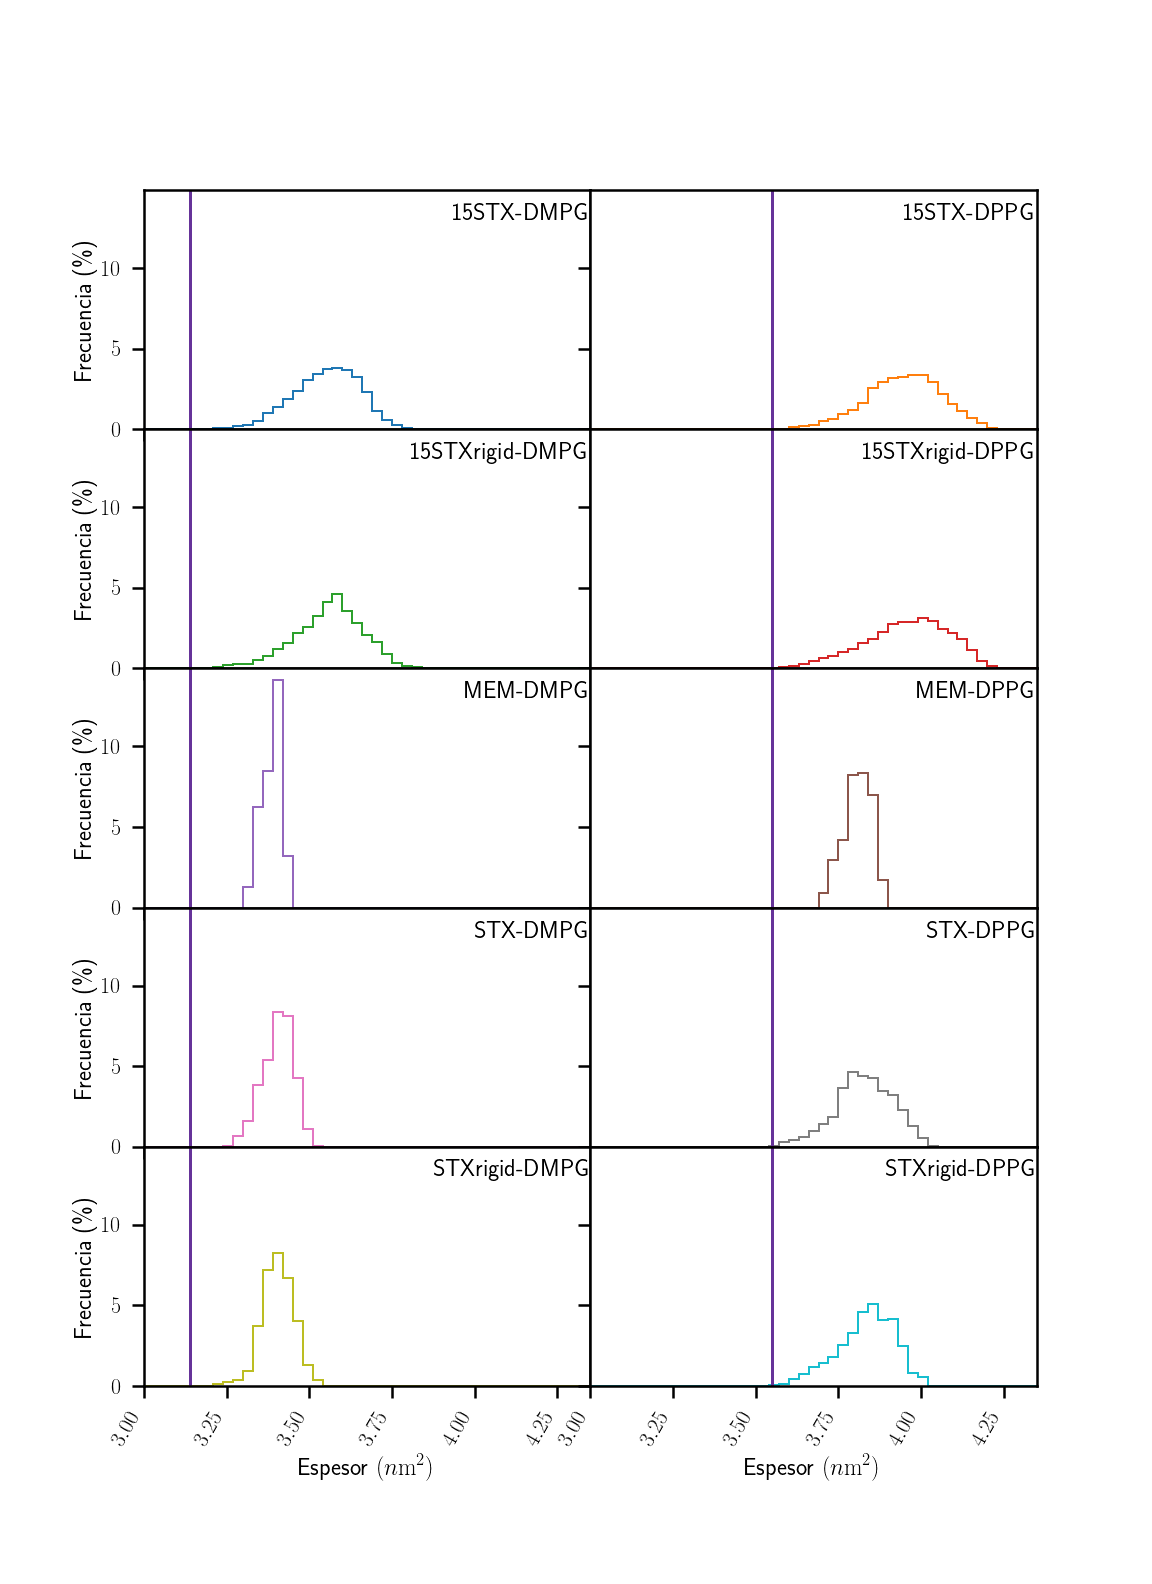
\includegraphics[scale=0.3,trim={0 3cm 0 6cm},clip]{Plots/thick_hist_g_lomepro.png}
  \caption{Distribuciones de los espesores locales hallados con g\_lomepro y para todos los sistemas. }
  \label{fig:thicglomepro}
\end{center}
\end{figure}

En la figura \ref{fig:aplthickglomepro} aparecen los valores promedio del \'{a}rea por l\'{i}pido en funci\'{o}n del espesor. Las etiquetas dicen la cantidad de estafiloxantina presente, \texttt{memb} significa que no hay, \texttt{1stx}  que hay una estafiloxantina, \texttt{15\%} que hay un 15 de estafiloxantina y \texttt{15\% rig} que el 15\% es para la mol\'{e}cula r\'{i}gida. Aparentemente en la figura se ve que entre mayor cantidad de estafiloxantinas disminuyen los valores promedio del \'{a}rea por l\'{i}pido y aumenta el espesor, sin embargo como las distribuciones del \'{a}rea por l\'{i}pido tienen un rango tan amplio,  los cambios en el \'{a}rea por l\'{i}pido no son significativos. Esta disminuci\'{o}n es coherente, ya que al disminuir el \'{a}rea por l\'{i}pido los componentes de la membrana tienden a compactarse, volvi\'{e}ndose m\'{a}s verticales y por consiguiente aumentando el espesor de la membrana.\\ 

\begin{figure}
\begin{center}
    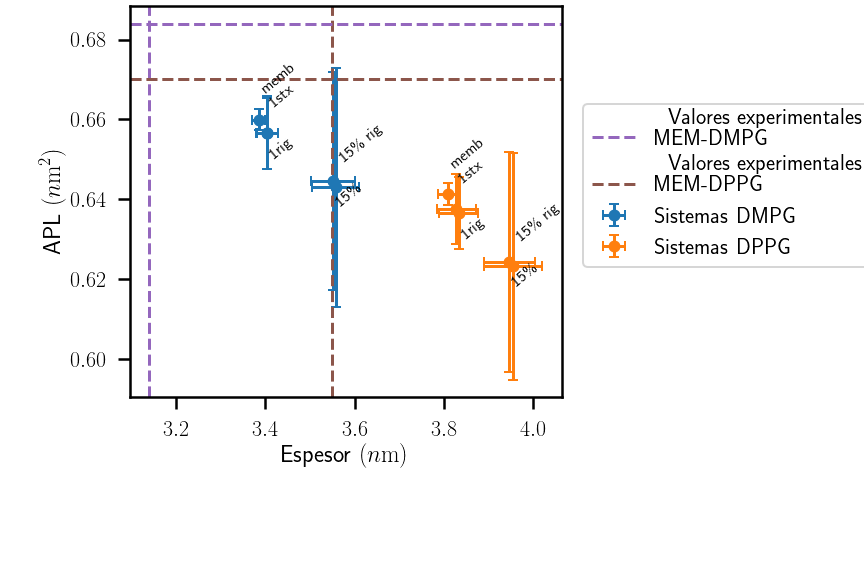
\includegraphics[scale=0.3,trim={0 3cm 0 0cm},clip]{Plots/apl_thickness.png}
  \caption{\'{A}reas locales por l\'{i}pido en funci\'{o}n de los espesores promedios locales hallados con g\_lomepro para todos los sistemas. Los puntos azules y amarillos son los valores promedio, mientras que las l\'{i}neas son los valores experimentales encontrados en \cite{Pan2012}. }
  \label{fig:aplthickglomepro}
\end{center}
\end{figure}

\section{Propiedades Globales de las Membranas Simuladas}
\subsection{Coeficiente de difusi\'{o}n}

En la gr\'{a}fica \ref{fig:msdlipid}, aparecen las desviaciones cuadr\'{a}ticas medias (msd) para los l\'{i}pidos sobre cada una de las r\'{e}plicas. As\'{i} mismo, en la figura \ref{fig:msdstx} aparecen los msd para las estafiloxantina y sobre cada una de las r\'{e}plicas. Para el caso de los l\'{i}pidos se observa una menor desviaci\'{o}n entre cada una de las r\'{e}plicas comparado con el caso de la estafiloxantina.\\ 

Con los datos de msd en funci\'{o}n del tiempo se buscaba hallar el coeficiente de difusi\'{o}n, debido a esto, no se han tenido en cuenta los primeros $100n\mathrm{s}$ que corresponden a la equilibraci\'{o}n del sistema. Luego se calcula el coeficiente de difusi\'{o}n de los l\'{i}pidos y de las estafiloxantinas considerando dos m\'{e}todos: En el primer m\'{e}todo se halla la constante a partir de un ajuste lineal tomando la trayectoria desde $100n$s hasta $400n$s y se descartan el primer 10\% ($0-30n$s) y el \'{u}timo 10\% ($370-400n$s), en el segundo m\'{e}todo se utilizan ventanas de tiempo de $40n$s, lo cual significa que se particiona la trayectoria en 6 fragmentos de $50n$s, son descartados los primeros y \'{u}ltimos 10\% de cada trayectoria, es decir, se descartan los primeros  y \'{u}ltimos $5n$s de cada uno de los 6 fragmentos, luego se promedian estas trayectorias y se les realiza un ajuste lineal. Las pendientes obtenidas se dividen en 4 de acuerdo a la ecuaci\'{o}n de Einstein, ecuaci\'{o}n \eqref{eq:diffei}. Todo el procedimiento es realizado con gromacs. Luego se promedian los coeficientes de difusi\'{o}n obtenidos en cada r\'{e}plica por los dos m\'{e}todos. El error est\'{a}ndar ha sido calculado sobre todas las r\'{e}plicas.\\

En la figura \ref{fig:dpbcinf} de la derecha aparece el coeficiente de difusi\'{o}n para una caja finita $D_{PBC}$ calculado con los dos m\'{e}todos. El primer m\'{e}todo aparece con puntos azules y amarillos, correspondiente al de la trayectoria completa. El segundo m\'{e}todo aparece con puntos verdes y rojos, correspondiente al m\'{e}todo de las ventanas de tiempo de $40n$s. Estos valores se contrastan con el coeficiente de difusi\'{o}n experimental para membranas de DMPG, encontrado a partir de una extrapolaci\'{o}n de los valores encontrados en \cite{Bag2014TemperatureSpectroscopy}. Cada uno de los valores graficados aparece en las tablas \ref{tab:dpbc} y \ref{tab:dinf} de los anexos.\\

\begin{figure}
\begin{center}
%trim={<left> <lower> <right> <upper>}
    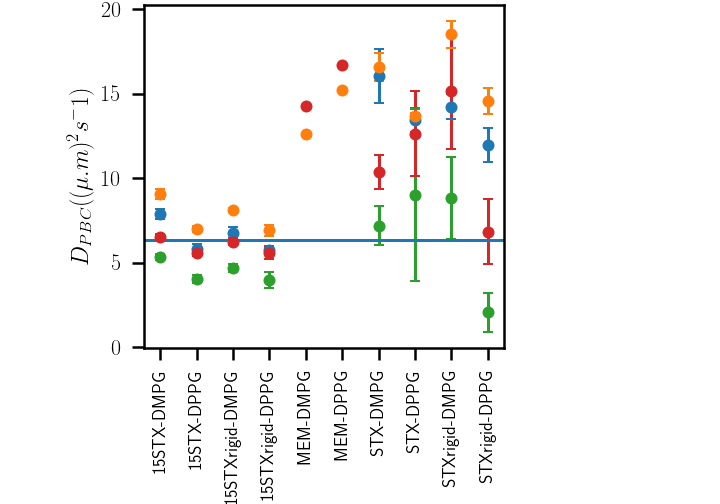
\includegraphics[scale=0.33,trim={0 0 5cm 0},clip]{Plots/diff_pbc.png}
    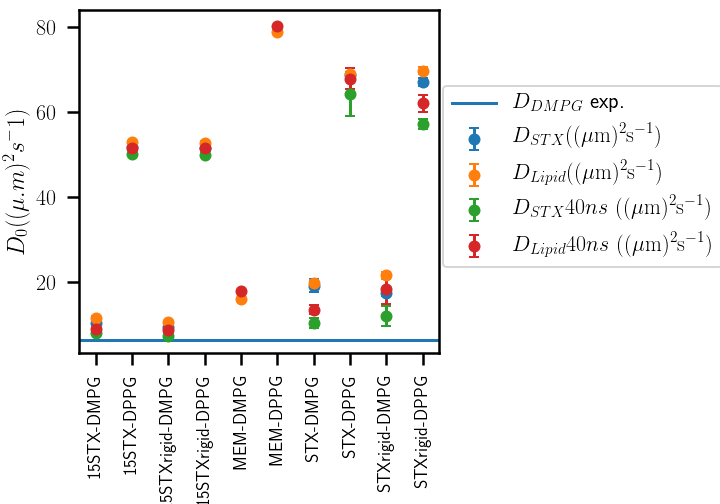
\includegraphics[scale=0.33]{Plots/diff_inf.png}
  \caption{\textit{Izquierda}: Coeficientes de difusi\'{o}n para una caja finita $D_{PBC}$ en condiciones de frontera peri\'{o}dicas. \textit{Derecha}: Coeficientes de difusi\'{o}n para una caja infinita. Obtenida seg\'{u}n la metodolog\'{i}a. Puntos azules y amarillos: M\'{e}todo de la trayectoria completa. Puntos verdes y rojos: M\'{e}todo de las ventanas de tiempo de $40n$s .}
  \label{fig:dpbcinf}
\end{center}
\end{figure}

Se observa que los coeficientes de difusi\'{o}n, calculados usando las trayectorias completas, son similares entre los sistemas DMPG y DPPG puros y los sistemas que contienen solo una mol\'{e}cula de STX (tanto para STX como STX r\'{i}gida). Todos estos valores fl\'{u}ctuan alrededor de 15$(\mu \mathrm{m})^2/s$ antes de ajustar para el tama\~{n}o de la caja. En presencia de 15\% de STX se observa una reducci\'{o}n notoria del coeficiente de difusi\'{o}n tanto para DMPG como para DPPG a un valor alrededor de los 5$(\mu \mathrm{m})^2/s$. Usando ventanas de tiempo de $40n$s se observa la misma diferencia en las constantes de difusi\'{o}n entre los sistemas puros y los sistemas con 15\% STX. Sin embargo, las mediciones de las constantes de difusi\'{o}n en presencia de una mol\'{e}cula de estafiloxantina presentan gran variabilidad e inconsistencia con los datos obtenidos con las ventanas de tiempo largas. Es necesario analizar estos datos con mas detalle para entender la fuente de estas fluctuaciones.\\

Tenemos que se cautelosos al comparar los datos de difusi\'{o}n para``MEM-DMPG'' y ``MEM-DPPG'' con los coeficientes de difusi\'{o}n cuando se inserta un 15\% de estafiloxantina. Seg\'{u}n V\"{o}gele et. al. \cite{Vogele2016DivergentMembranes}, el coeficiente de difusi\'{o}n depende de las dimensiones de la caja usadas durante la simulaci\'{o}n bajo condiciones peri\'{o}dicas. En nuestro caso tanto MEM-DMPG como MEM-DPPG contienen 128 l\'{i}pidos y las simulaciones con 15\% STX  contienen 362 l\'{i}pidos m\'{a}s 64 estafiloxantinas. Se ajustan los coeficientes proyectando a una caja de tama\~{n}o infinito usando la ecuaci\'{o}n \eqref{eq:diffinf}. En la ecuaci\'{o}n se requieren las dimensiones de la caja y las viscosidades cinem\'{a}ticas de los l\'{i}pidos a $T=323$K. Las dimensiones de la caja fueron obtenidas con gromacs y las viscosidades utilizadas correspoden a las de los l\'{i}pidos dimiristoil fosfatidilcolina (DMPC) y dipalmitoil fosfatidilcolina (DPPC) encontradas en Nojima et. al. \cite{Nojima2014ViscositySpectroscopy}.\\

\begin{figure}
\begin{center}
    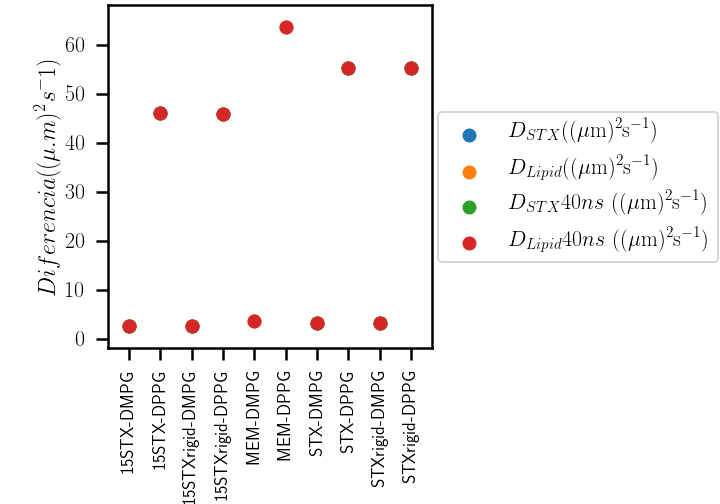
\includegraphics[scale=0.35]{Plots/differences.png}
  \caption{Diferencia entre los coeficientes de difusi\'{o}n de la caja peri\'{o}dica y la caja infinita.}
  \label{fig:ddiff}
\end{center}
\end{figure}
Como los coeficientes de difusi\'{o}n para la caja infinita dependen del coeficiente de viscosidad de la membrana y como no se utilizaron los valores correctos de viscosidad para fosfatidilgliceroles, entonces tambi\'{e}n se ha calculado el cambio relativo entre el coeficiente de difusi\'{o}n para la caja infinita con respecto al coeficiente de difusi\'{o}n de la caja finita. Para esto, sea $D_0$ el coeficiente de la caja infinita y sean $D_1$ y $D_2$ los coeficientes de difusi\'{o}n para dos cajas de diferentes tama\~{n}os, por ejemplo, una caja de 128 l\'{i}pidos y otra de 362 l\'{i}pidos, entonces el cambio relativo entre los dos tama\~{n}os de la caja puede definirse como:
\begin{equation}
\Delta=\frac{D_1-D_0}{D_1-D_0}    
\end{equation}
De la ecuaci\'{o}n \eqref{eq:diffinf}, se encuentra que este cambio relativo es:
\begin{equation}\label{eq:delta}
\frac{D_1-D_0}{D_2-D_0}=\frac{L_{z2}\left[\frac{3}{2}\ln{\left(\frac{L_{x1}}{L_{z1}}\right)}-\xi_{xx}\right]}{L_{z1}\left[\frac{3}{2}\ln{\left(\frac{L_{x2}}{L_{z2}}\right)}-\xi_{xx}\right]}
\end{equation}
Usando el lado derecho de la expresi\'{o}n \eqref{eq:delta}, tomando $L_{x1}, L_{z1}$ como las dimensiones de las cajas de 128 l\'{i}pidos y $L_{x2}, L_{z2}$   como las dimensiones de las cajas de los otros sistemas, se puede ver en la gr\'{a}fica \ref{fig:delta} que el cambio relativo entre los coeficientes de difusi\'{o}n es mayor a 1. Esto significa que independientemente de la confiabilidad de los par\'{a}metros de la viscosidad cinem\'{a}tica, el coeficiente de difusi\'{o}n disminuye.\\
\begin{figure}
\begin{center}
    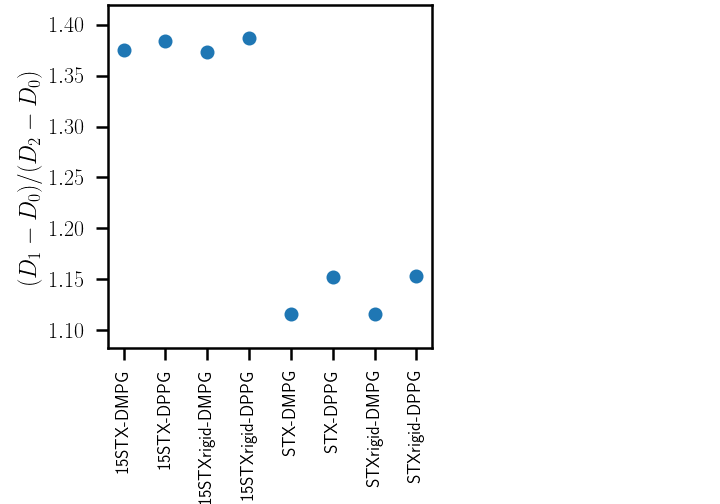
\includegraphics[scale=0.35]{Plots/quotient.png}
  \caption{Diferencia relativa entre los coeficientes de difusi\'{o}n de la caja peri\'{o}dica y la caja infinita.}
  \label{fig:delta}
\end{center}
\end{figure}


A pesar de que la correcci\'{o}n para una caja infinita produce un aumento en los coeficientes de difusi\'{o}n mayor para los sistemas que tienen estafiloxantina, tambi\'{e}n es posible ver que hay una disminuci\'{o}n en el coeficiente de difusi\'{o}n significativa cuando a los sistemas de la membrana pura se les inserta un 15\% de estafiloxantina.\\

\subsection{Perfil de estr\'{e}s}
El perfil de estr\'{e}s se ha calculado para todas las r\'{e}plicas y luego se han explorado varias opciones para obtener informaci\'{o}n sobre cada sistema. El perfil de estr\'{e}s corresponde a presiones positivas y negativas en funci\'{o}n del eje vertical y representa las fuerzas atractivas o repulsivas moleculares que mantienen la estabilidad de la membrana. Se esperan valores positivos en las cabezas polares debido a repulsiones electrost\'{a}ticas y valores negativos atractivos relacionados a las cadenas aciles, en particular en la regi\'{o}n interfacial donde son m\'{a}s fuertes las interacci\'{o}nes cohesivas debido a la exclusi\'{o}n entr\'{o}pica de mol\'{e}culas de agua en esta zona. Debido al ruido que presentan las curvas (correspondiente a la sombra de color gris) y  a las asimetr\'{i}as que estas presentan, respecto al centro de la membrana, se aplica sobre las curvas un filtro gaussiano de 2 desviaciones est\'{a}ndar y tambi\'{e}n se aplica uno de 4.\\

Las curvas sin filtar y promediadas se encuentran en el anexo \ref{AnexoB}. Mientras que las curvas con el filtro gaussiano de 2 aparecen en la figura \ref{fig:stress2}. Estas curvas adem\'{a}s se han simetrizado, es decir, se han promediado los valores que est\'{a}n a los lados derecho e izquierdo de la membrana.\\
\begin{figure}
\begin{center}
    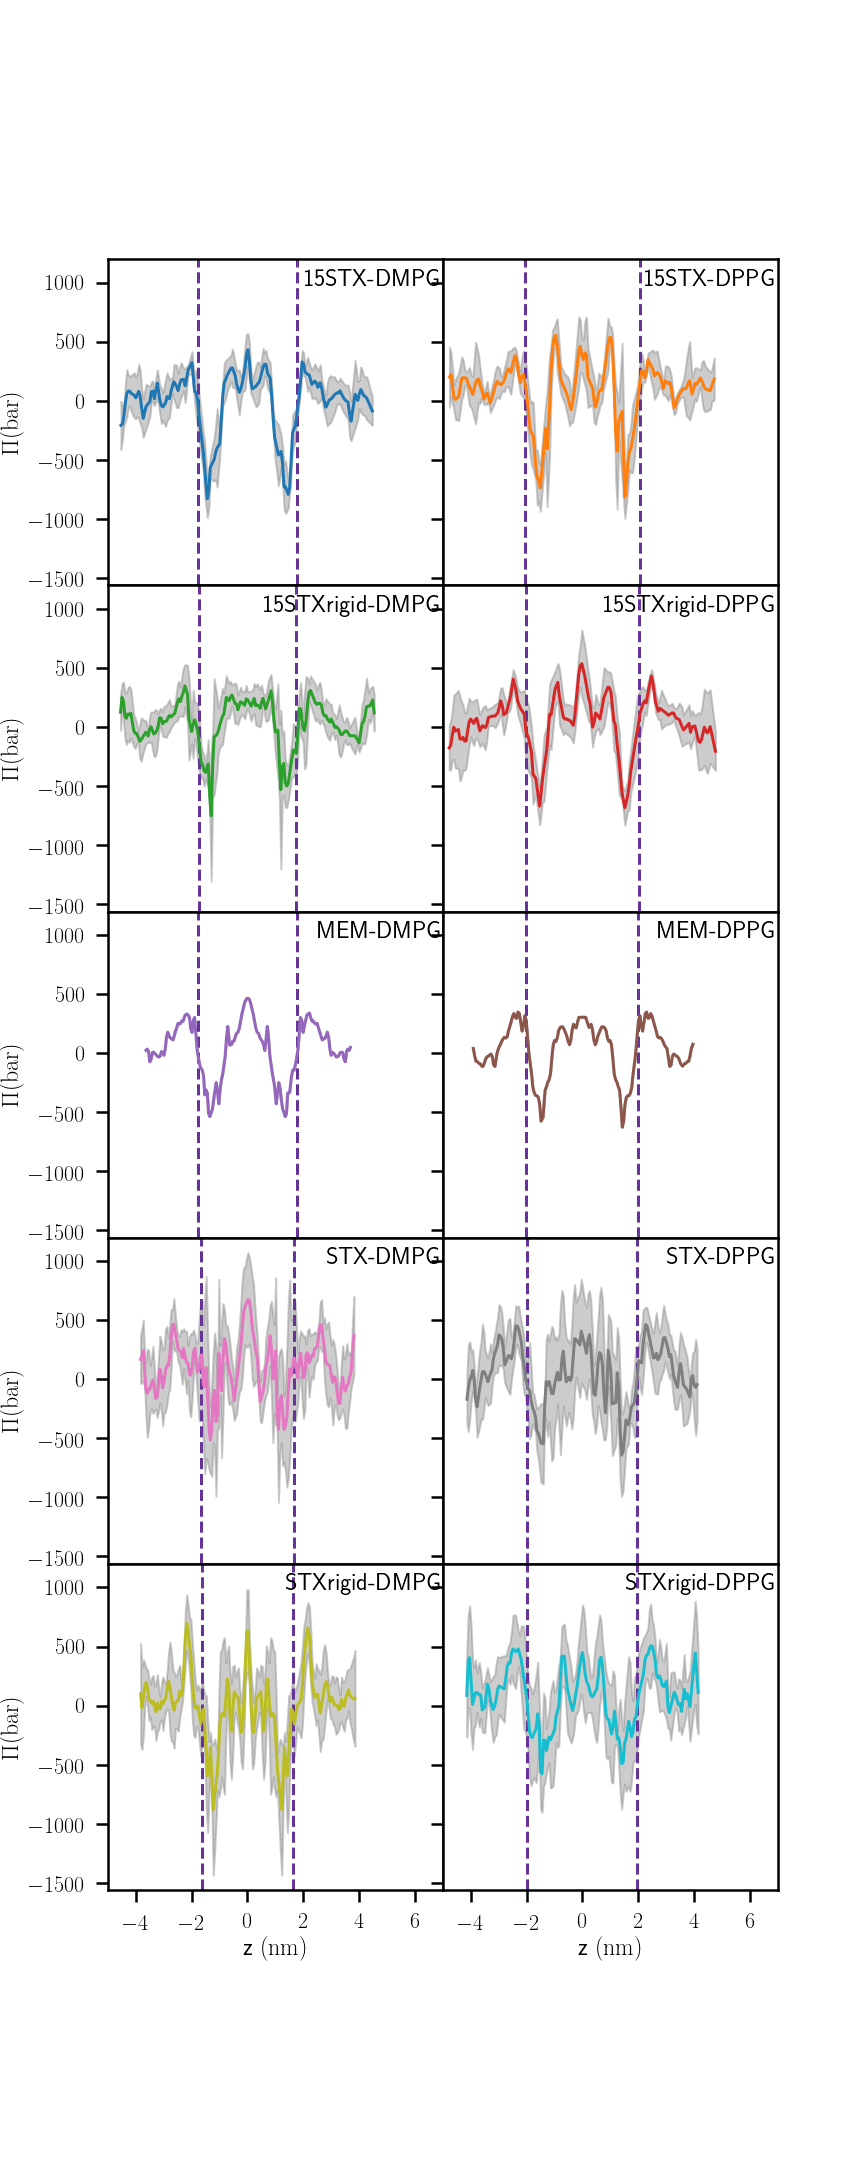
\includegraphics[scale=0.25,trim={0 6cm 0 9cm},clip]{Plots/stress_profile_2_sym.png}
  \caption{Perfil de estr\'{e}s promediado para todas las r\'{e}plicas con un filtro gaussiano de 2. Las l\'{i}neas punteadas representan la posici\'{o}n de los grupos fosfato. }
  \label{fig:stress2}
\end{center}
\end{figure}
En la figura \ref{fig:stress2}, la l\'{i}nea punteada representa la posici\'{o}n de los grupos fosfato hallada mediante la herramienta de gromacs. De acuerdo a la literatura \cite{Vanegas2011CrystallineErgosterol}, los dos m\'{a}ximos positivos del perfil de presi\'{o}n (picos positivos) corresponden a la posici\'{o}n de los grupos fosfato, esto es debido a la repulsi\'{o}n electrost\'{a}tica entre los f\'{o}sforos, los cuales poseen cargas ani\'{o}nicas, lo cual induce un trabajo positivo sobre el sistema, sin embargo, en la figura \ref{fig:stress2} la posici\'{o}n de los grupos fosfato de gromacs aparece desplazada hacia el centro respecto a los picos correspondientes..\\

Los dos m\'{i}nimos globales del perfil de presi\'{o}n (valles negativos) son valores negativos puesto que se deben a interacciones favorables entre los grupos apolares de la membrana debido a interacciones hidrof\'{o}bicas, \cite{Vanegas2011CrystallineErgosterol} y que usualmente corresponden a interacciones en la interfaz hidrof\'{i}lica/hidrof\'{o}bica de la membrana. Los dos valles encontrados son acordes a los resultados de \cite{Vanegas2011CrystallineErgosterol}, ya que los dos valles son m\'{a}s notorios cuando la membrana est\'{a} en la fase l\'{i}quida desordenada $L_{\alpha}$.\\

Al mirar el rango de valores que toma el perfil de presi\'{o}n, se encuentra que este toma principalmente valores negativos, esto puede deberse a que la membrana est\'{e} sometida a estr\'{e}s por el solvente, el cual debe inducir presiones positivas (repulsivas) en la interface que no est\'{a}n siendo contabilizadas en el perfil de presi\'{o}n lip\'{i}dico. Cabe aclarar que el perfil de estr\'{e}s es negativo en los resultados mostrados por \cite{Vanegas2011CrystallineErgosterol} cuando la membrana se encuentra en fase gel. Tambi\'{e}n hay otras simulaciones \cite{Vanegas2014ImportanceSimulations} en que las presiones negativas aparec\'{i}an mayoritariamente en simulaciones de grano grueso (en ingl\'{e}s \textit{coarse grained simulations}). Este es el primer intento, seg\'{u}n nuestro conocimiento, en generar un perfil de estr\'{e}s sobre membranas ani\'{o}nicas de PGs y podr\'{i}a ser una caracter\'{i}stica intr\'{i}nseca del sistema PG el tener perfiles de presi\'{o}n netamente negativos. Adem\'{a}s, existe una relaci\'{o}n entre el perfil de estr\'{e}s y la tensi\'{o}n superficial de la membrana: Esta tensi\'{o}n superficial es crucial en mantener la estabilidad de la membrana y ciertos estudios \cite{Losasso2019ModulationBilayers} proponen que la reducci\'{o}n en la tensi\'{o}n superficial en la presencia de p\'{e}ptidos antimicrobiales favorece la formaci\'{o}n de poros ya que reduce la barrera energ\'{e}tica para inducir estos poros. Es importante notar que los perfiles de presi\'{o}n que reportamos en este trabajo de tesis son preliminares ya que debemos confirmar en estudios posteriores, que los ajustes aplicados con el fin de reducir ruido son v\'{a}lidos.\\

A continuaci\'{o}n presentamos un esquema para calcular la tensi\'{o}n superficial de la membrana con base en la integral del perfil de estr\'{e}s:
\begin{equation}
    \gamma=-\int_{z_1}^{z_2}z\Pi(z)\mathrm{d}z.
\end{equation}
Como la tensi\'{o}n superficial $\gamma$ y la curvatura $c_0$ est\'{a}n directamente relacionadas mediante el m\'{o}dulo de flexi\'{o}n $\kappa_c$:
\begin{equation}
    \gamma=\kappa_c c_0,
\end{equation}
entonces el perfil de estr\'{e}s se relaciona con la curvatura:
\begin{equation}
    \kappa_{c}c_0=-\int_{z_1}^{z_2}z\Pi(z)\mathrm{d}z.
\end{equation}
Dado que el perfil de estr\'{e}s toma valores mayoritariamente negativos, entonces se espera que la membrana posea una curvatura positiva. Sin embargo, no consideramos prudente reportar valores de tensi\'{o}n superficial en esta tesis hasta que no  validemos los c\'{a}lculos realizados.\\

Comparando los perfiles de presi\'{o}n entre los sistemas que no tienen estafiloxantina y los que s\'{i} la tienen no se encuentran cambios  en el orden de magnitud entre los picos y los valles de los perfiles de presi\'{o}n. Entre las diferencias presentadas est\'{a} que cuando solo se inserta una estafiloxantina, el perfil de presi\'{o}n presenta m\'{a}s ruido, en cambio cuando la concentraci\'{o}n de estafiloxantina es del 15\% se vuelve a estabilizar el perfil de presi\'{o}n. Tambi\'{e}n se observan diferencias en los patrones de perfil de presi\'{o}n en el centro de la membrana para cada sistema, para los sistemas de membranas puras tiende a aparecer un \'{u}nico pico positivo que hace referencia a una repulsi\'{o}n en la membrana, en cambio en los sistemas con una estafiloxantina empiezan a aparecer m\'{a}s picos y valles, hasta que a un 15\% de estafiloxantina, en especial para 15\%STX en DMPG y 15\%STX r\'{i}gido en DMPG los picos desaparecen. En este momento ser\'{i}a prematuro dar una interpretaci\'{o}n biof\'{i}sica al efecto de la estafiloxantina en la modulaci\'{o}n de los perfiles de presi\'{o}n hasta no validar la estrategia de correcci\'{o}n de las curvas.\\ 

